%!TEX root = ../thesis.tex
%*******************************************************************************
%****************************** Second Chapter *********************************
%*******************************************************************************

\chapter{General physical properties 2D materials \label{chap:3}}

\ifpdf
    \graphicspath{{Chapter3/Figs/Raster/}{Chapter3/Figs/PDF/}{Chapter3/Figs/}{Chapter3/Figs/Vector/}}
\else
    \graphicspath{{Chapter3/Figs/Vector/}{Chapter3/Figs/}}
\fi

In this thesis, the properties of materials are virtually divided into preliminary and advanced categories. In this chapter, we will focus on the preliminary properties of 2D materials, namely structural, electronic, vibrational and mechanical properties. These properties are considered as test calculations and knowledge which the advanced properties in the next chapter are closely related to. They are composed of both my original calculations and results from literatures. An emphasis will be made on the characteristic properties of 2D materials.

\section{Structural properties}
\subsection{Layer structure}

As has seen in the \fullref{chap:1}, layered materials have a closest relationship with 2D materials. The strong anisotropic structure in the former results in the layer concept. This anisotropic nature attributes to the weak interlayer bonding and the strong intralayer bonding. The van der Waals interaction (vdWs)\cite{vdws} is the main type of this weak bonding. vdWs is the attraction and repulsion between atoms or molecules entities caused by dipole-dipole, dipole-induced dipole and instantaneous induced dipole-induced dipole forces. The definition is sometimes extended to include other weak forces between molecules as well.  For the 2D materials, vdWs interaction become important as the number of layers becomes larger than one: few-layer materials with typical number of layers less than ten. They also belong to the 2D materials family since the thickness of the materials still small such that quantum confinements still play role. As in its layered bulk part, a few-layer system is stacked of monolayers that hold together through vdWs. When no other bonding types are presented, interlayer vdWs determines all the change brought by going above single layer and its impact on the electronic structure will be significant. For example, as going from monolayer to bilayer, the linear dispersion relation of energy $E$ and momentum $k$ evolves into parabolic-like spectrum\cite{Partoens2006,Mak2010}. 

\begin{figure}[htbp!] 
\centering  
\includegraphics[width=0.8\textwidth]{gra_band.png}
\caption{Energy-momentum dispersion relation of single layer and bilayer graphene as plane intersections of 3D graphite dispersion. Image adapted from: \cite{Mak2010}. }  
\label{fig:gra_bands}
\end{figure} 

In \autoref{fig:gra_bands} (a), the dispersion relation in graphite along the z direction, that is the HKH line in the Brillouin zone, is shown in blue plane. This direction is perpendicular to the graphite layers. Because of the interlayer interaction and quantum confinements, in few-layer system, the finite thickness limits the number of wave vectors that standing waves can take.  Therefore, if only the intralayer and interlayer interactions between nearest neighbour atoms were considered, the dispersion relations in few-layer systems could be considered as the dispersions on the corss-section of red planes that cut the graphite Brillouin zone, see \autoref{fig:gra_bands} (a).  These planes are perpendicular to the z direction and intersect with the HKH line at possible points. This is called the zone-folding of dispersion relations\cite{saito1998physical}. These points are illustrated in \autoref{fig:gra_bands} (b). Under the condition that quantum confinements at few-layer system require the wave functions vanish at the imaginary layer outside the surface of the system, the systems will have well-defined wave vectors. Then, the dispersion relations will be on the plane intersects at $k_z=\pi/c$ and at $kz=2(\pi/3c)$ for graphene and bilayer graphene, respectively.  Having the knowledge of 3D band structure of graphite, we can approximate the dispersion of few-layer systems in this way. As a result, as shown in red plane in \autoref{fig:gra_bands} (a) and their 3D version in \autoref{fig:gra_bands} (c), graphene has linear dispersion relations and bilayer graphene has parabolic-like two dispersion bands. Moreover, the bilayer structure will never pass through the H point where graphene has passed and have linear dispersion relation. This is because of standing waves in bilayer will have a wave vector $k=2(n \pi/3c)$, where $n$ is a positive integer: 1, 2, ... , n. This will not equal to $\pi/c$ for any number of $n$. More generally, systems with an even number of layers will not have linear dispersion; whereas systems with an odd number of layers always have linear dispersion relation. Further, if other interactions were considered, an overlap of bands those touch each other in (c) would happened\cite{Partoens2006}. This overlap increases with the number of layers. Eventually in graphite, maximum overlap is reached.


\begin{figure}[htbp!] 
\centering  
\includegraphics[width=0.8\textwidth]{mos2_band.png}
\caption{Energy-momentum dispersion relation of single layer and bulk graphene as plane intersections of 3D graphite dispersion. Image adapted from: \cite{Mak2010b}. }  
\label{fig:mos2_band}
\end{figure} 

Another example of the importance of interlayer interaction in the few-layer 2D materials will the MoS$_2$. As mentioned in the \fullref{chap:1}, as going from bulk to monolayer, MoS$_2$ transforms from an indirect band gap to a direct one. Here again we can make use of zone-folding to approximate the band structure of monolayer from layered bulk one. The monolayer and the layered structure of 2H phase is shown in \autoref{fig:mos2_band} (a). In (b) let us focus on the difference of dispersion relations on the planes parallel to the page passing through K$\Gamma$ and HA lines (simply call them K$\Gamma$ and HA planes below). Same as the graphite, 2H layered MoS$_2$ has two layers per unit cell. Therefore, according to the standing wave arguments that we have used for graphene above, HA plane represents the monolayer. $E_g$ and $E\prime_g$ are the band gap of monolayer and layered bulk structures. Here not only the magnitude of band gap increased as going from bulk to monolayer, character of the band gap has changed as well. It is shown that this is due to the band edges change. Interlayer interactions widen top valence bands at $\Gamma$ and bottom conduction band at the middle of $\Gamma$K line, which without interlayer interaction should be degenerated. Therefore, these two band edges become the ones those determine the band gap instead of band edges at $K$ in the monolayer. Contrast to this, band edges at $K$ are not effected too much by the interlayer interaction to make a difference. When we compare the difference between band edges of K and other two is, we could find out that the latter two have much larger contribution from p$_z$ orbitals that give maximum interlayer orbital overlap hence interlayer interaction than d orbitals that dominant at $K$ point.


\subsection{sp hybirdization}

When atoms come together form bonds, the orientations of these bonds are decisive for the final structure. The sp hybridization is a good example of this.  It can mainly exist in three different variants: sp, sp$^2$ and sp$^3$, see \autoref{fig:sp_hybrid}. The hybridization index $n$ in sp$^n$ stands for the relative amount of p character in the hybridization. For example, sp$^2$ has 1/3 s character and 2/3 p character. Hybridized bonds  tend to maximized their distance to reduce the energy raised by the repulsion of electrons. As shown in \autoref{fig:sp_hybrid}, this results in tetrahedral structure of diamond that made of sp$^3$ bonds, trigonal planar structure of graphite or graphene that made of sp$^2$ and linear structure of ethyne molecules that made of sp bonds.  \citet{coulson1949} generalized the relation of bond angle and $n$ in the following way:

\begin{equation}
1=-\sqrt{n_1n_2}~cos\theta_{12}, 
\end{equation}

where $\theta_{12}$ is the bond angle between orbital 1 and 2. The bond angle can be measured in atomic simulations, yet we still need one more constrain to solve the equation for $n$ if orbital 1 and 2 have different $n$. This constrain is that, in the case of carbon atom, the total fractions of all s hybridized orbitals should equal 1, while it should be 3 for the sum of the p fractions. Consequently, each bond from one atom can be assigned with a unique $n$. This formula is useful to determine the s and p composition of the bonds. For example, $\theta_{12}=90^o$ gives $n\rightarrow\infty$, which means it is pure p orbital; $\theta_{12}=120^o$ gives $n=2$, that is a sp$^2$ bond. Generally, wider bond angle corresponds to large s contribution. Of course, this is more useful when the bond angle takes value other than those three types of hybridized bonds mentioned. Then we can use it to explain resulting geometrical structure.

\begin{figure}[htbp!] 
\centering  
\includegraphics[width=0.8\textwidth]{sp_hybrid.png}
\caption{Three types of sp hybridizaton. Image adapted from: \cite{sp_hybrid}. }  
\label{fig:sp_hybrid}
\end{figure} 


\section{Electronic properties}

Electronic properties is one of the first feature we usually like to know about the new materials. Not only it is because semiconductor and metal have different role in applications, but also because the details of the electronic structure set the direction towards which further exploration should be carried out. One example for this from my experience is that from monitoring the electronic structure variations we had predicted how the mobility of the carrier can be tuned. This will be discussed in the later chapter. Therefore, it is important to understand this property of a new material to fully reveal its potentials. Electronic properties usually characterized by band structure (BS) and density of states (DOS). These calculations are standard calculations in first-principles codes where all consequent calculations start. After solving the Kohn-Sham equation with proper cut-off energy, k points etc., we will have all eigenenergy of each state identified with k point in the Brillouin zone and band index.  DOS is a count of the number of states at specific energy. BS is the plot of eigenenergy verse the line in Brillouin zone that connects high symmetry k points.  2D material has vast variation of electronic properties. From semimetallic graphene to semiconducting MoS$_2$ and to insulating BN. We have already seen these in the introduction. The purpose of this section is to point out some of the interesting electronic properties of some 2D materials. We will start with a introduction to the electronic properties of graphene alone with some concept can be used later, such as orbital, hybridization etc..

The number of valence electrons in C atom is four (two core electrons are inert for chemical bonding thus excluded). Each C atom has three sp$^2$ bonds that lead to the honeycomb structure of graphene. The $p_z$ orbital left unchanged and have one electron. The results of bonding is shown in \autoref{fig:gra_bonds}. One $sp2$ hybridized orbital with another one from adjacent atom form strong $\sigma$ bond, while $p_z$ orbitals form $\pi$ bonds. It may look like an alternative single and double bonds between atoms, actually the bond order in graphene is 4/3 and it is uniform. We will talk about how a delocalized $\pi$ bond is more stable than alternative single and double bonds in the later chapter where Clar's theory is discussed.

\begin{figure}[htbp!] 
\centering  
\includegraphics[width=\textwidth]{double_bond}
\caption{The formation of $sp^2$ $\sigma$ and $p_z$ $\pi$ double bond. Image source: \cite{gra_bond}. }  
\label{fig:gra_bonds}
\end{figure} 



\begin{figure}[htbp!] 
\centering  
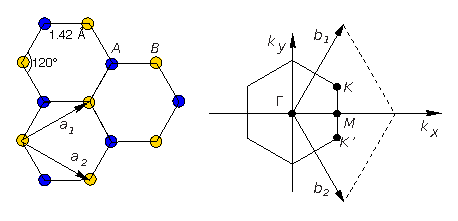
\includegraphics[width=\textwidth]{gra_lat.eps}
\caption{Graphene lattice and its Brillion zone. Image source: \cite{CastroNeto2009}. }  
\label{fig:gra_lat}
\end{figure} 

Every atom has same local environment, however, adjacent atoms are not equivalent. They belong to different hexagonal sublattices $A$ and $B$ as indicated with blue and yellow colors in \autoref{fig:gra_lat}. $a_1$ and $a_2$ are the basis vectors in real space connecting equivalent sites. $b_1$ and $b_2$ are the basis vectors in reciprocal space connecting equivalent k-points. The hexagon in the reciprocal space is the first Brillouin zone where all inequivalent k-points are contained. These kpoints associate with different parallel lines of atoms and thus also indicate different directions in the real space. The k wave vectors near the $\Gamma$ point have longer wave length, while those at the boundary of the first Brillouin zone have wave length that is two times the unitcell dimension on that direction. For example, the most interesting k-point for graphene is the $K$ and $K'$ points. These directions correspond to the $a_1$ and $a_2$ directions in real space. It is only at these k-points in the Brioulloin zone, the antibinding and bonding $\pi$ band touch each other. 



As compared to $\pi$ bond, $\sigma$ bond originate from strong overlap of $sp^2$ orbitals. The interaction is strong and the splitting of bonding and antibonding orbitals are large. Which makes the $\sigma$ bonding orbitals deep in energy, or in other word, makes it strong and difficult to break. This feature contribute the most to the mechanical strength of graphene. On the other hand, $p_z$ orbitals are less overlapped. This makes the $pi$ bond energy close to Fermi level, i.e. the highest occupied state. Therefore, they contribute the most to the electronic properties of graphene.  



\subsection{Dirac materials}

We have seen that graphene, silicene and germanene have an interesting electronic structure: Dirac cone. We also have listed the consequences of having such fearture: high mobility, massless carrier etc.. In this section, we will discuss the symmetry condition for the existence of Dirac cones. This knowledge is useful to find more materials of this type. 

According to von Neumann-Wigner theorem, the space-time inversion symmetry is crucial for the existence and protection of Dirac cones\cite{Wang2015b}. It is a combination of space inversion and time reversal symmetries. These two are equally important and has to act simultaneously for the possible formation of Dirac cones. More restrict condition that guarantee the existence of Dirac cones has to deal with relations of hopping integrals\cite{Hasegawa2006,Liu2013}. It is from the \citet{Liu2013}'s study that it revealed the hexagonal lattice has the most favourable structure to posses Dirac cones. The probability decreases as one goes from hexagonal to square lattice, as shown in \autoref{fig:dirac_hs}.

\begin{figure}[htbp!] 
\centering  
\includegraphics[width=0.95\textwidth]{dirac_hs.png}
\caption{Possible positions of second atom (blue area) to guarantee the existence of Dirac cones as going from (a) square lattice to (f) hexagonal lattice. The first atom is located at the corners of the unit cell. Image source: \cite{Liu2013}. }  
\label{fig:dirac_hs}
\end{figure} 

\subsection{Polar bond}
\subsection{Importance of crystal symmetry}



\subsection{Accurate description from DFT}

\section{Vibrational properties}
\subsection{Phonon dispersion of 2D materials}
\subsection{Dynamic stability from phonon dispersion}

\section{Mechanical properties}
\subsection{Elastic and engineering constants}
\subsection{Mechanical stability: Born stability criteria}